\section{Rounds 2--3: IRT-accelerated search}\label{sec:r2}
The first round used the full 110-item fitness for every candidate (about 1{,}000\,s of generation each), which left no budget for EvoGM's outer loop. To continue the search under a further 8-GPU-hour cap, we resumed the saved search state and replaced most full evaluations with a cheaper estimate.

\paragraph{IRT subset and estimator.} The 40 round-1 candidates $\times$ 110 items form a correctness matrix (truncated $=$ wrong). We fit a 2PL item-response model per task (MMLU-Pro, GPQA, BFCL) by joint MAP ($\theta\sim\mathcal N(0,1)$, $\log a\sim\mathcal N(0,0.5^2)$, $b\sim\mathcal N(0,2^2)$) and kept, per task, the items with the highest Fisher information at the abilities of the top-15 candidates divided by $\sqrt{\text{mean tokens}}$: 16 MMLU-Pro + 10 GPQA + 14 BFCL $=$ 40 items (about 66k generated tokens per candidate instead of about 165k). A new candidate answers only these 40 items. Per task, its fitness estimate is the observed number correct on the subset plus the sum of the 2PL probabilities $p(\theta_{\text{MAP}})$ over the unobserved items, divided by the task size; the three task values are averaged, so the estimate is on the same scale as the round-1 fitness. In leave-one-out validation over the 40 round-1 candidates the estimate had a mean absolute error (MAE) of 0.013 against the full fitness (0.009 on the top 15) and a rank correlation of 0.93; the naive subset accuracy had an MAE of 0.066.

\paragraph{Racing.} Outputs are streamed while a candidate is generating. Once at least half of the subset has finished, the controller computes an optimistic estimate ($\theta+1.5\,\text{sd}$) and stops the candidate if it falls below the current $P$-th best population value. In an offline simulation on round-1 iterations 2--3 this pruned 4 of 20 candidates, saved about 9\% of the time and pruned none wrongly.

\paragraph{Completion rule.} To guard against estimation error and the winner's curse, after every iteration the two best not-yet-completed population members are evaluated on the 70 missing items (one per GPU) whenever the best one's estimate is within 0.02 of the best exact fitness so far. This gives their exact 110-item fitness under the round-1 definition. The population and the generators use the best available value (exact if known, otherwise the estimate). The final winner is the candidate with the highest \emph{exact} 110-item fitness over round 1 and all completions; only that candidate is run on the 180-item test.

\paragraph{Search schedule.} Each new round starts with a basis shift: the top-8 candidates of the previous round's history become the new experts (round 2: fitness .722, .703, .697, .697, .692, .692, .689, .686), and the search runs in their coordinates with $P=10$, a fresh generator per round and up to three iterations per round. Rounds and iterations were sized inside the kernel from the measured costs, always reserving time for the final test.

\section{Rounds 2--3: results}\label{sec:r2res}
\paragraph{Run.} The run finished in 6.53 GPU hours on 2$\times$T4 (cap 8\,h). It completed rounds 2 and 3 with three iterations each; round 4 was skipped because the remaining 0.88\,h was less than the 0.92\,h a round needs at minimum. It made 64 new subset evaluations (104 candidates in total with round 1) and 12 completions; 3 candidates were stopped early by racing and none failed.

\paragraph{Search trajectory.} The best exact fitness stayed at the round-1 value 0.722 through round 2 (one completed candidate tied it), rose to 0.733 in round 3, iteration 2, and to 0.764 in round 3, iteration 3 (Figure~\ref{fig:search}, left). Across the 12 completed candidates the IRT estimate had an MAE of 0.009 against the exact fitness, a Spearman correlation of 0.96, and a mean bias of $+0.008$ (Figure~\ref{fig:search}, right). The bias is expected: completions are chosen because their estimates are high. The winner shows it most clearly, with an estimate of 0.782 and an exact fitness of 0.764.

\begin{figure}[htbp]
\centering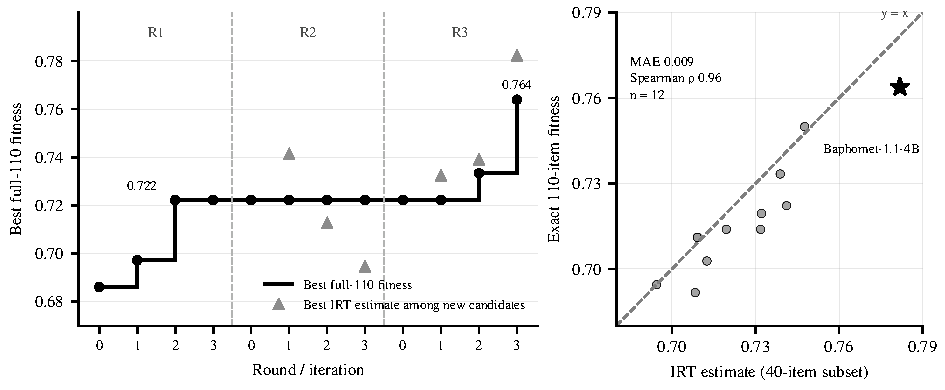
\includegraphics[width=\textwidth]{fig_search_r2_en.pdf}
\caption{Left: best exact 110-item fitness so far after each iteration of rounds 1--3 (iteration 0 $=$ initial population of the round); triangles: best IRT estimate among the new candidates of that iteration (rounds 2--3). Right: IRT estimate vs.\ exact 110-item fitness for the 12 completed candidates; the star is Baphomet-1.1-4B.}
\label{fig:search}
\end{figure}

\paragraph{Baphomet-1.1-4B coefficients.} The round-3 winner is
\begin{align*}\lambda_{1.1} = (&0.0116,\ 0.2039,\ 0.5901,\ 0.0013,\ 0.2972,\ 0.0323,\ 0.0030,\ -0.0007)\end{align*}
over (Agents-A1, dsv4pro, q38distill, Qwopus-Coder, Qwopus-v3, AREX-Turbo, NeoHorse, T-Max), $\sum\lambda_i=1.14$. Compared with the round-1 winner it keeps the same three donors but moves weight from q38distill (0.63\,$\to$\,0.59) to dsv4pro (0.10\,$\to$\,0.20) and Qwopus-v3 (0.23\,$\to$\,0.30); the other five donors stay near zero (Figure~\ref{fig:lambda}).

\begin{figure}[htbp]
\centering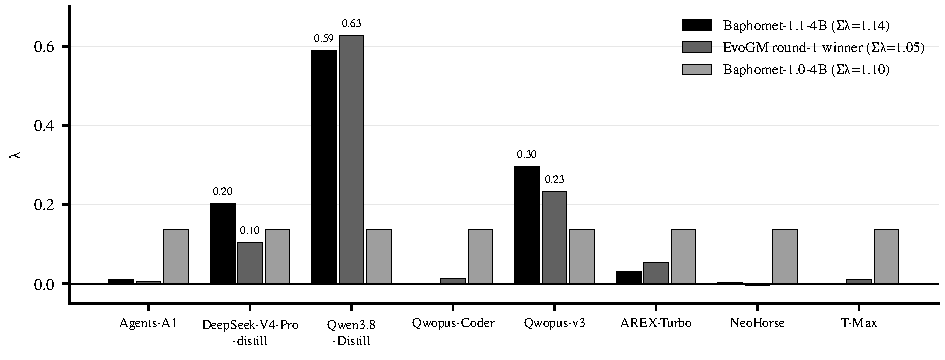
\includegraphics[width=\textwidth]{fig_lambda_en.pdf}
\caption{Merge coefficients of Baphomet-1.1-4B, the round-1 winner and Baphomet-1.0-4B.}
\label{fig:lambda}
\end{figure}

\paragraph{Comparison with the experts on the fitness set.} Table~\ref{tab:fit110} and Figures~\ref{fig:fit110}--\ref{fig:fit110eff} compare Baphomet-1.1 with the eight donors, the uniform average, Baphomet-1.0 and the round-1 winner on the 110 fitness items (4{,}096-token cap). Baphomet-1.1 has the highest fitness (0.764), 0.078 above the best single donor (q38distill, 0.686) and 0.161 above Baphomet-1.0 (0.603); it is first or tied for first on MMLU-Pro (.800) and GPQA (.567), while AREX-Turbo is higher on BFCL (.950 vs.\ .925). Two cautions apply. Baphomet-1.1 was \emph{selected} on these items, so its score is optimistically biased; the donors' scores are not. The donors were evaluated only on this set and \emph{not} on the 180-item test.

\begin{table}[htbp]
\centering\small
\caption{110-item fitness set (4{,}096-token cap). Fit.\ $=$ mean of the three task accuracies; Trunc.\ $=$ share of truncated answers (\%); Tok.\ $=$ mean completion tokens. Baphomet-1.1 and the round-1 winner were selected on these items (optimistic); donors were not run on the 180-item test.}
\label{tab:fit110}
\setlength{\tabcolsep}{4pt}
\begin{tabular}{lcccrrr}
\toprule
Model & MMLU & GPQA & BFCL & Fit. & Trunc. & Tok. \\
\midrule
\textbf{Baphomet-1.1-4B} & .800 & .567 & .925 & \textbf{.764} & 11.8 & 1{,}149 \\
Round-1 winner & .800 & .467 & .900 & .722 & 12.7 & 1{,}096 \\
\midrule
q38distill & .700 & .433 & .925 & .686 & 3.6 & 671 \\
dsv4pro & .675 & .467 & .850 & .664 & 19.1 & 1{,}331 \\
Qwopus-v3 & .700 & .233 & .925 & .619 & 27.3 & 1{,}835 \\
Qwopus-Coder & .650 & .167 & .875 & .564 & 33.6 & 1{,}834 \\
NeoHorse & .600 & .033 & .900 & .511 & 40.0 & 2{,}180 \\
T-Max & .500 & .133 & .900 & .511 & 41.8 & 2{,}343 \\
AREX-Turbo & .425 & .067 & .950 & .481 & 28.2 & 1{,}924 \\
Agents-A1 & .450 & .067 & .750 & .422 & 48.2 & 2{,}492 \\
\midrule
Baphomet-1.0-4B & .650 & .233 & .925 & .603 & 31.8 & 1{,}925 \\
Uniform average ($1/8$) & .675 & .200 & .900 & .592 & 30.9 & 2{,}073 \\
\bottomrule
\end{tabular}
\end{table}

\begin{figure}[htbp]
\centering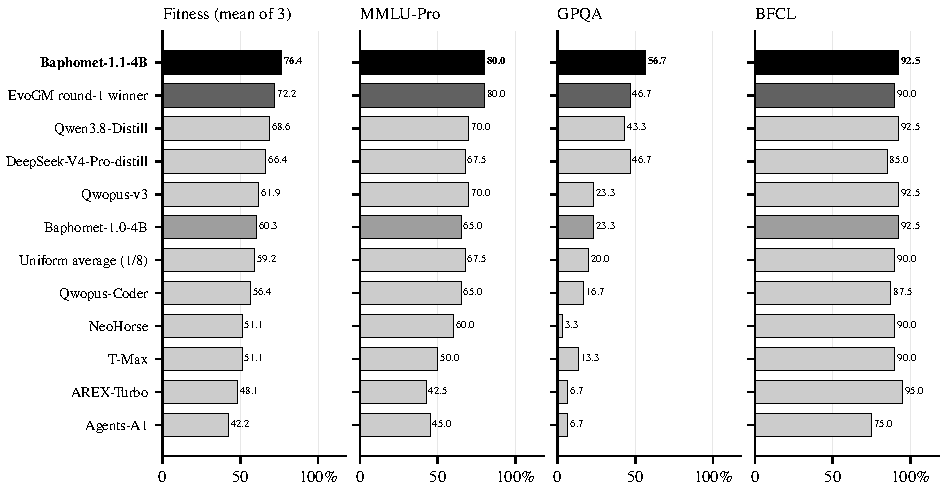
\includegraphics[width=\textwidth]{fig_fit110_acc_en.pdf}
\caption{Fitness and per-task accuracy on the 110-item fitness set for Baphomet-1.1-4B, the round-1 winner, the eight donors, Baphomet-1.0-4B and the uniform average. Baphomet-1.1 was selected on these items, so its score is optimistic.}
\label{fig:fit110}
\end{figure}

\begin{figure}[htbp]
\centering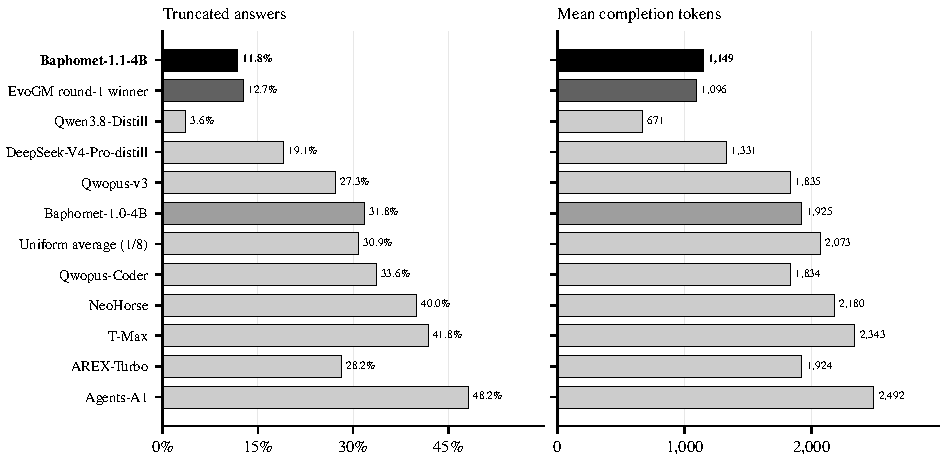
\includegraphics[width=\textwidth]{fig_fit110_eff_en.pdf}
\caption{Truncation rate and mean completion tokens on the 110-item fitness set (same models and order as Figure~\ref{fig:fit110}).}
\label{fig:fit110eff}
\end{figure}

\paragraph{Test set.} Table~\ref{tab:test} and Figure~\ref{fig:test} give the 180-item results for the four models run on the test (the donors and the uniform average were not). Baphomet-1.1 is numerically best overall (79.4\%, Wilson 95\% CI 73.0--84.7) ahead of Baphomet-1.0 (77.8\%, 71.2--83.2), the round-1 winner (77.2\%, 70.6--82.7) and Qwen3.5-4B (70.0\%, 62.9--76.2). The intervals overlap widely. In the paired test (Table~\ref{tab:mcnemar}) Baphomet-1.1 is \emph{not} significantly better than Baphomet-1.0 (10 items won, 7 lost, $p=0.63$) or than the round-1 winner (12 vs.\ 8, $p=0.50$), and is significantly better than the base model (20 vs.\ 3, $p<0.001$), mainly through GPQA (10 vs.\ 0, $p=0.002$) and MMLU-Pro (9 vs.\ 1, $p=0.021$). Per suite against Baphomet-1.0 it is ahead on MMLU-Pro (+3.8 points) and GPQA (+4.0) and behind on BFCL ($-4.0$, 0 vs.\ 2 discordant items), none significant.

\begin{table}[htbp]
\centering\small
\caption{180-item test (8{,}192-token cap). Acc.\ in \%; Trunc.\ $=$ share of truncated answers (\%); Tok.\ $=$ mean completion tokens. Donors were not run on this test.}
\label{tab:test}
\setlength{\tabcolsep}{4pt}
\begin{tabular}{llrrr}
\toprule
Suite ($n$) & Model & Acc. & Trunc. & Tok. \\
\midrule
MMLU-Pro (80) & \textbf{Baphomet-1.1-4B} & \textbf{81.3} & 5.0 & 1{,}492 \\
 & Round-1 winner & 75.0 & 5.0 & 1{,}200 \\
 & Baphomet-1.0-4B & 77.5 & 13.8 & 3{,}331 \\
 & Qwen3.5-4B & 71.3 & 17.5 & 4{,}385 \\
\midrule
GPQA (50) & \textbf{Baphomet-1.1-4B} & \textbf{62.0} & 28.0 & 4{,}007 \\
 & Round-1 winner & 62.0 & 16.0 & 3{,}270 \\
 & Baphomet-1.0-4B & 58.0 & 34.0 & 5{,}915 \\
 & Qwen3.5-4B & 42.0 & 54.0 & 7{,}094 \\
\midrule
BFCL (50) & \textbf{Baphomet-1.1-4B} & 94.0 & 0.0 & 207 \\
 & Round-1 winner & 96.0 & 0.0 & 202 \\
 & Baphomet-1.0-4B & \textbf{98.0} & 0.0 & 205 \\
 & Qwen3.5-4B & 96.0 & 0.0 & 229 \\
\midrule
All (180) & \textbf{Baphomet-1.1-4B} & \textbf{79.4} & 10.0 & 1{,}834 \\
 & Round-1 winner & 77.2 & 6.7 & 1{,}498 \\
 & Baphomet-1.0-4B & 77.8 & 15.6 & 3{,}180 \\
 & Qwen3.5-4B & 70.0 & 22.8 & 3{,}983 \\
\bottomrule
\end{tabular}
\end{table}

\begin{table}[htbp]
\centering\small
\caption{Paired comparison on the 180-item test: items only the first model got right -- items only the second got right, and the exact two-sided McNemar $p$.}
\label{tab:mcnemar}
\setlength{\tabcolsep}{4pt}
\begin{tabular}{lcccc}
\toprule
Comparison & All & MMLU-Pro & GPQA & BFCL \\
\midrule
Baphomet-1.1 vs.\ Baphomet-1.0 & 10--7 ($p$=.63) & 5--2 (.45) & 5--3 (.73) & 0--2 (.50) \\
Baphomet-1.1 vs.\ round-1 winner & 12--8 (.50) & 7--2 (.18) & 5--5 (1.0) & 0--1 (1.0) \\
Baphomet-1.1 vs.\ Qwen3.5-4B & 20--3 ($<$.001) & 9--1 (.021) & 10--0 (.002) & 1--2 (1.0) \\
Round-1 winner vs.\ Baphomet-1.0 & 8--9 (1.0) & 3--5 (.73) & 5--3 (.73) & 0--1 (1.0) \\
Baphomet-1.0 vs.\ Qwen3.5-4B & 17--3 (.003) & 7--2 (.18) & 9--1 (.021) & 1--0 (1.0) \\
\bottomrule
\end{tabular}
\end{table}

\begin{figure}[htbp]
\centering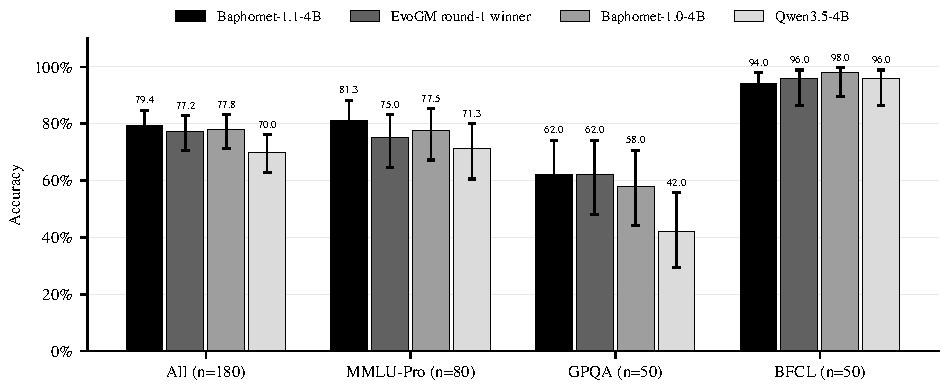
\includegraphics[width=\textwidth]{fig_test180_acc_en.pdf}
\caption{180-item test accuracy with Wilson 95\% confidence intervals (8{,}192-token cap). Only these four models were run on the test; the eight donors and the uniform average were not.}
\label{fig:test}
\end{figure}

\paragraph{Reasoning length.} Baphomet-1.1 generates 42\% fewer completion tokens than Baphomet-1.0 overall (1{,}834 vs.\ 3{,}180; 55\% fewer on MMLU-Pro, 32\% fewer on GPQA) and truncates less (10.0\% vs.\ 15.6\%). Compared with the round-1 winner, however, it is longer (1{,}834 vs.\ 1{,}498 tokens) and truncates more (10.0\% vs.\ 6.7\%), almost entirely on GPQA (28\% vs.\ 16\% truncated; Figure~\ref{fig:testeff}). Part of the accuracy gain over the round-1 winner was therefore bought with longer reasoning.

\begin{figure}[htbp]
\centering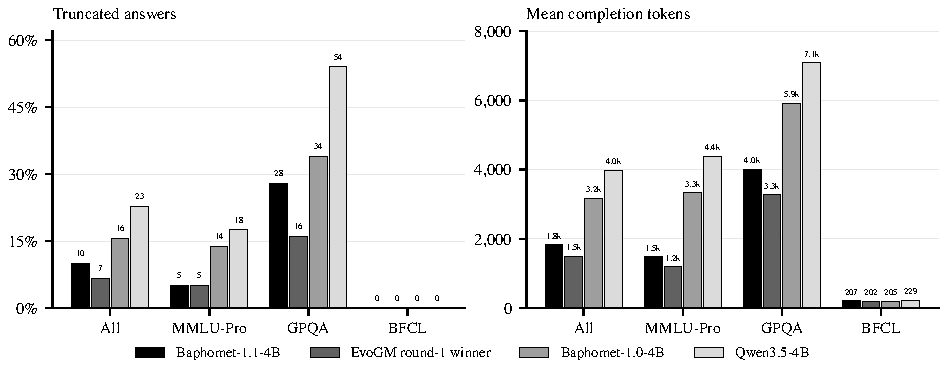
\includegraphics[width=\textwidth]{fig_test180_eff_en.pdf}
\caption{Truncation rate and mean completion tokens on the 180-item test.}
\label{fig:testeff}
\end{figure}

